\documentclass[12pt]{extarticle}
\usepackage[utf8]{inputenc}
\usepackage[legalpaper, portrait, margin=0.8in]{geometry}
\usepackage{amssymb}
\usepackage{amsmath}
\usepackage{graphicx}

\title{CDA5106 - Advanced Computer Architecture \\ Final Exam Review}
\author{Kobee Raveendran}
\date{}

\begin{document}
    \maketitle

    \section{Module 1: High-Performance Microprocessor Architecture}

    \subsection{Module 1.2: Power Wall and Dennard Scaling}

    \subsubsection{Notes}

    \begin{itemize}
        \item energy: ability of a physical system to do work on other physical systems (unit: joule)
        \item power: rate at which energy is transformed (unit: watt; 1 watt = 1 joule delivered per second)
        
        \begin{itemize}
            \item power = $V \cdot I$ (V = voltage, I = current)
        \end{itemize}
        
        \item for capacitors:
        
        \begin{itemize}
            \item energy stored = $0.5 \cdot C \cdot V^2$ (C = capacitance, V = voltage)
            \item if a capacitor is drained at a frequency of $f$ per second: 
            power = $\frac{energy}{second} = 2 \cdot 0.5 CV^2 = CV^2$
        \end{itemize}

        \item Power wall problem
        \begin{itemize}
            \item $P_{dyn} = ACV^2f$
            \item A: fraction of gates actively switching
            \item C: total capacitance of all gates
            \item V: supply voltage
            \item f: frequency of switching
        \end{itemize}

        \item Power wall fundamentals
        \begin{itemize}
            \item max frequency vs. threshold voltage:
            \item $f_{max} = c \cdot \frac{(V - V_{thd})^{1.3}}{V}$
        \end{itemize}

        \item \textbf{Dennard Scaling Example (old)}
        \begin{itemize}
            \item if gate length (transistor size) scales by $S = 0.7$ (both length and width), then:
            \item capacitance scales by $S = 0.7$
            \item original area scales by $S^2 = 0.5$
            \item number of transistors scales by $\frac{1}{S^2} \approx 2$
            \item supply voltage ($V$) scales by $S = 0.7$
            \item frequency ($f$) scales by $\frac{1}{S} = 1.4$
            \item then, \textbf{dynamic power} $P_{dyn} = ACV^2f$
            \item and \textbf{new dynamic power} $P_{dyn}' = A'C'V'^2f'$
            \item $P_{dyn}' = (2A)(0.7C)(0.7V)^2(1.4f) \approx 1 \cdot ACV^2f = P_{dyn}$
        \end{itemize}

        \item \textbf{Post Dennard Scaling example (new)}
        \begin{itemize}
            \item capacitance scales by $S = 0.7$
            \item number of transistors scales by $\frac{1}{S^2} = 2$
            \item supply voltage ($V$) cannot scale without also scaling threshold voltage ($V_{thd}$), and doing that 
            increases static power exponentially
            \item frequency ($f$) scales by $\frac{1}{S} = 1.4$
            \item result: dynamic power doubles every generation
            \item $P_{dyn} = ACV^2f$
            \item $P_{dyn}' = A'C'V'^2f' = (2A)(0.7C)(1 \cdot V)^2(1.4f) \approx 2 \cdot P_{dyn}$
        \end{itemize}

        \subsubsection{Exercises}

			\begin{enumerate}
				\item Suppose that instead of progressing at a ratio of 0.7, Moore’s law slows down and transistor gate length scales at a ratio of 0.8 instead. Find the dynamic power consumption under \textit{unlimited} and \textit{limited} scaling for the next process generation.

				\begin{itemize}
					\item Unlimited/old scaling rule
					\begin{itemize}
						\item gate length scales by $S = 0.8$
						\item capacitance scales by $S = 0.8$
						\item original area scales by $S^2 = 0.64$
						\item num transistors thus scales by $\frac{1}{S^2} = 1.56$
						\item supply voltage scales by $S = 0.8$
						\item frequency scales by $\frac{1}{S} = 1.25$
						\item dynamic power stays constant:
					
						$P_{dyn} = (1.56A)(0.8C)(0.8V)^2(1.25f)$
					\end{itemize}
					
					\item leakage-limited/new scaling
					\begin{itemize}
						\item capacitance scales by $S = 0.8$
						\item num transistors scales by $\frac{1}{S^2} = 1.56$
						\item supply voltage does not scale without scaling threshold voltage too, which increases static power exponentially
						\item frequency scales by $\frac{1}{S} 1.25$
						\item dynamic power consumption increases:

						$P_{dyn}' = (1.56A)(0.8C)(V)^2(1.25f) = 1.56 \cdot P_{dyn}$
					\end{itemize}
				\end{itemize}

				\item With limited voltage scaling, suppose that we want to keep the dynamic power consumption constant in the next generation by keeping frequency constant and reduce die area. How much should we reduce die area to achieve that?
				\begin{itemize}
					\item gate length scales by $S = 0.7$
					\item capacitance scales by $S = 0.7$
					\item original area scales by $S^2 = 0.5$
					\item supply voltage and frequency are constant
					\item dynamic power consumption must stay constant: $P_{dyn}' = P_{dyn}$

					$ACV^2f = A'(0.7C)V^2f \longrightarrow A = 0.7A'$

					\item number of transistors in the next generation: $A' = 1.4A$ (instead of 2A like before; i.e. 70\% of 2A)
					\item thus die area shrinks by 30\%
				\end{itemize}

				\item Describe the difference between energy and power.

				Power is the rate of energy consumption.

				\item Describe the impact of threshold voltage choice on static and dynamic power consumption as transistors are scaled down.

				If threshold voltage is lowered, dynamic power decreases (nearly linearly) but static power increases exponentially.

				\item How has processor design adapted to the power wall problem?

				Stalling frequency growth, multicore, and sophisticated power management (clock gating, voltage and frequency scaling, power gating).
			\end{enumerate}

    \end{itemize}

	\subsubsection{Overview of ILP Techniques}

	Caches example

	\begin{itemize}
		\item processor with 1-ns clock
		\item 64KB cache memory with 2-ns read time, 95\% hitrate
		\item 512MB main memory with 150-ns read time
		\item What is the average access time (AAT) in this memory system?
	\end{itemize}

	Answer:
	\begin{itemize}
		\item hits: $95 \cdot 2$ ns, misses: $5 \cdot (2 + 150)$ ns
		\item total = hit time + miss time = $190 + (10 + 750) = 950 ns$
		\item AAT = $\frac{total}{100} = 9.5ns$
	\end{itemize}

	\section{Module 2: Performance, Cost, and Reliability of Microprocessors}

	\subsection{Performance Evaluation 1}

	\subsubsection{Amdahl's Law}

	\begin{itemize}
		\item performance improvement (``speedup'') is limited by the part you can't improve
		\item (s) $Speedup_{enhanced} =$ best case speedup from gizmo alone
		\item (f) $Fraction_{enhanced} =$ fraction of task that gizmo can enhance
		\item $s_{overall} = \frac{1}{(1 - f) + \frac{f}{s}}$
	\end{itemize}

	Example:

	\begin{itemize}
		\item jet plane wing simulation, where 1 run takes 1 week on your computer
		\item your program is 80\% parallelizable
		\item new supercomputer has 100,000 processors
		\item $s = 100,000$
		\item $f = 0.8$
		\item overall speedup: $s_{overall} = \frac{1}{(1 - f) + \frac{f}{s}} = \frac{1}{(1 - 0.8) + \frac{0.8}{100000}} \approx \frac{1}{0.2} = 5$
		\item only about 5 times faster (33 hours instead of 1 week), but not worth the high price tag (using a cheaper computer with only 100 processors instead yields a 4.8X speedup!)
	\end{itemize}

	More examples:

	Ex 1:

	\begin{itemize}
		\item $f = 0.95$
		\item $s = 1.10$
		\item $s_{overall} = \frac{1}{(1-0.95) + \frac{0.95}{1.10}} = 1.094 \approx 1.10$
	\end{itemize}

	Ex 2:

	\begin{itemize}
		\item $f = 0.05$
		\item $s \rightarrow \infty$
		\item $s_{overall} = 1.053$
	\end{itemize}

	\subsubsection{Run Time}

	\begin{itemize}
		\item CPU time = clock cycle count $\times$ cycle time
		\item cycles per instruction (CPI) = $\frac{\texttt{clock cycle count}}{\texttt{instruction count}}$
		\item CPU time = IC $\times$ CPI $\times$ CT
	\end{itemize}

	\subsection{Performance Evaluation 2}

	Determine speedup by comparing program times with respect to a reference machine.

	

	\begin{itemize}
		\item arithmetic mean (which one should we trust?):
		
		\begin{tabular}[h!]{|c|c|c|c|} \hline
					   & Computer A & Computer B & B vs. A   \\ \hline
			Program P1 & 2X faster  & 4X faster  & 2X faster \\ \hline
			Program P2 & 5X faster  & 15X faster & 3X faster \\ \hline
			Average	   & 3.5X		& 9.5X		 &			 \\ \hline
		\end{tabular}

		Speedups:

		\begin{itemize}
			\item method 1: program-wise $\longrightarrow \frac{2 + 3}{2} = 2.5$X faster
			\item method 2: machine-wise $\longrightarrow \frac{9.5}{3.5} = 2.71$X faster
		\end{itemize}

		\item geometric mean (consistent):
		
		$\displaystyle gmean = \sqrt[n]{\prod_{i = 1}^n} = exp(\frac{\frac{1}{n} \sum_{i=1}^n \ln (x_i)}{n})$

		\begin{tabular}[h!]{|c|c|c|c|} \hline
					   & Computer A 	& Computer B 	& B vs. A   	\\ \hline
			Program P1 & 2X faster  	& 4X faster  	& 2X faster 	\\ \hline
			Program P2 & 5X faster  	& 15X faster 	& 3X faster 	\\ \hline
			Average	   & $\sqrt{10}$	& $\sqrt{60}$	& $\sqrt{6}$	\\ \hline
		\end{tabular}

		Speedups:

		\begin{itemize}
			\item method 1: program-wise $\longrightarrow$ B is $\sqrt{2 \cdot 3} = \sqrt{6}$X faster
			\item method 2: machine-wise $\longrightarrow$ B is $\sqrt{60} \cdot \sqrt{10} = \sqrt{6}$X faster
		\end{itemize}

		\item (also important): geometric standard deviation
		
		$\displaystyle gstdev = exp(\sqrt{\frac{\prod_{i=1}^n (\ln x_i - \ln gmean)^2}{n}})$

		in plain English: for each ``component'' speedup vs. ref machine, take its natural log and subtract the natural 
		log of the gmean from that. Square it and multiply all of these together, then divide by n. Finally take the 
		square root of this, then take $e$ to the power of the result.
	\end{itemize}

	\subsubsection{Exercises}

	Given the following table of speedups for machines A and B relative to a reference machine:

	\begin{tabular}[h!]{|c|c|c|c|} \hline
		Prog	& X (secs)	& A (secs)	& B	(secs)	\\ \hline
		App 1	& 30		& 15		& 10		\\ \hline
		App 2	& 20		& 15		& 10		\\ \hline
		App 3	& 40		& 20		& 30		\\ \hline
		App 4	& 15		& 20		& 15		\\ \hline
	\end{tabular}

	Compute the following (see post-computation table below to find them all):

	\begin{itemize}
		\item geometric speedup of machine A vs. base machine X
		
		from the table, we find that A has a 1.41X speedup over X

		\item geometric speedup of machine B vs. base machine X
		
		from the table, we find that B has a 1.68X speedup over X

		\item geometric speedup of machine B vs. machine A
		
		from the table, we find that B has a 1.19X speedup over A

		\item geometric standard deviation of the speedup of machine A over machine X
		
		$gstd = exp(\sqrt{\frac{1}{4} \cdot \ln^2(\frac{2}{1.41}) \ln^2(\frac{1.33}{1.41}) \ln^2(\frac{2}{1.41}) \ln^2(\frac{0.75}{1.41})})$

		$gstd = 1.002255... \approx 1$

	\end{itemize}

	\begin{tabular}[h!]{|c|c|c|c|} \hline
		Prog		& A vs. X	& B vs. X	& B vs. A	\\ \hline
		App 1		& 2X		& 3X		& 1.5X		\\ \hline
		App 2		& 1.33X		& 2X		& 1.5X		\\ \hline
		App 3		& 2X		& 1.33X		& 0.67X		\\ \hline
		App 4		& 0.75X		& 1X		& 1.33X		\\ \hline
		\bf{Product}& 4X		& 8X		& 2X		\\ \hline
		\bf{gmean}	& 1.41X		& 1.68X		& \bf{1.19X}\\ \hline
	\end{tabular}

	\subsection{Cost and Reliability}

	\subsubsection{Failure Rates ($\lambda$)}

	\begin{itemize}
		\item $\lambda$ = the number of failures that occur per unit time in a component/system
		\item FIT (failure in time) = number of failures in $10^9$ hours
		\item example: 10,000 microprocessor chips used for 1,000 hours, and 8 of them fail. Failure rate is thus 
		$\frac{8}{10,000 \cdot 1,000} = 8 \cdot 10^{-7}$ (failures per hour per chip) $\cdot 10^9$ hours = 800 FITs
	\end{itemize}

	\subsubsection{Reliability Metrics}

	\begin{itemize}
		\item $R(t)$ = probability that the system still works correctly at time $t$
		\item $W_N(t)$ = number of items (of the same kind) that would still be working at time $t$
		\item if $\lambda$ is constant, then $R(t) = e^{-\lambda t}$
		\item Mean Time Between Failure (MTBF) = $\frac{1}{\lambda}$
	\end{itemize}

	\subsubsection{System Reliability}

	Assume that:

	\begin{itemize}
		\item $M$ components are in the system with failure rates $\lambda_1, \lambda_2, ..., \lambda_m$
		\item for the system to work properly, all components must also work properly
		\item a component's reliability is independent of any other component's reliability
		\item then, system failure rate = sum of component's failure rates
		\item $R_{sys}(t) = R_1(t) \cdot R_2(t) \cdot ... \cdot R_m(t) = e^{-\lambda_1 t \cdot ... \cdot -\lambda_mt}$
		$= e^{-(\lambda_1 + \lambda_2 + ... + \lambda_m)t} = e^{-\lambda_{sys}t}$
	\end{itemize}

	Other metrics:

	\begin{itemize}
		\item Mean Time To Repair (MTTR): mean time to repair/recover from a fault
		\item Mean Time Between Failure (MTBF): mean time between 2 consecutive failures
		\item if each failure is repaired, then MTBF = MTTF + MTTR
		\item usually, MTTF $\gg$ MTTR, so MTBF and MTTF are often interchangeable
	\end{itemize}

	\subsubsection{Examples}

	Assume a disk subsystem with:

	\begin{itemize}
		\item 10 disks each rated at $10^6$-hour MTTF
		\item 1 SCSI controller rated at $5 \cdot 10^5$-hour MTTF
		\item 1 power supply rated at $2 \cdot 10^5$-hour MTTF
		\item 1 fan rated at $2 \cdot 10^5$-hour MTTF
		\item 1 SCSI cable rated at $10^6$-hour MTTF
	\end{itemize}

	Find the failure rate of the entire disk subsystem.

	$R_{sys}(t) = 10 \cdot \frac{1}{10^6} + \frac{1}{5 \cdot 10^5} + \frac{2}{2 \cdot 10^5} + \frac{1}{10^6}$
	$			= \frac{10 + 2 + 5 + 5 + 1}{10^6} = \frac{23}{10^6} = \frac{23,000}{10^9} = 23,000$ FIT

	Thus, MTTF = $\frac{1}{\lambda_{sys}} = \frac{1}{23,000} \cdot 10^9 \approx 43,500$ hours

	\section{Instruction Set Design}

	\subsection{Instruction Set Architecture 1}

	\subsubsection{Styles of ISAs}

	\begin{itemize}
		\item Stack:
		\begin{itemize}
			\item \texttt{push <addr>, pop <addr>} (or ALU instructions)
			\item ALU: pop two entries, perform ALU operation, push result onto stack
			\item compact instruction format
			\begin{itemize}
				\item all calculation operations take 0 operands
				\item flexible; used for compiling Java bytecode (not dependent on registers in architecture [but all 
				have stacks])
			\end{itemize}
		\end{itemize}

		\item Accumulator:
		\begin{itemize}
			\item \texttt{load/store/ALU <addr>} (result affects accumulator register)
			\item also very compact (all operations take 1 operand, the other is implicitly the accumulator register)
			\item less dependence on memory than stack-based
		\end{itemize}

		\item Register-memory:
		\begin{itemize}
			\item \texttt{load/store/ALU <reg>, <reg/addr>}
			\begin{itemize}
				\item at most one operand can be a memory address
				\item leftmost register is the destination (if applicable)
			\end{itemize}
		\end{itemize}

		\item Load-Store:
		\begin{itemize}
			\item \texttt{load/store <reg>, <addr>}
			\item ex: \texttt{ALU <reg1>, <reg2>, <reg3>}: reg1 is destination, other 2 are source registers
		\end{itemize}
	\end{itemize}

	Example for adding two numbers:

	\begin{tabular}[ht!]{|c|c|c|c|} \hline
		Stack	& Accumulator	& Register-memory	& Load-Store	\\ \hline
		push A	& load A		& load R1 A			& load R1 A		\\ \hline
		push B	& add B			& add R1 B			& load R2 B		\\ \hline
		add		& store C		& store C R1		& add R3 R1 R2	\\ \hline
		pop C	& 				& 					& store C R3	\\ \hline
	\end{tabular}

	Pros/cons:

	\begin{itemize}
		\item load-store
		\begin{itemize}
			\item (+) fixed length instructions possible (allows for easy fetch/decode)
			\item (+) simpler hardware: efficient pipeline and potentially lower cycle time
			\item (-) higher instruction count
			\item (-) fixed-length instructions can be wasteful (more bits than needed for some instructions)
		\end{itemize}

		\item register-memory
		\begin{itemize}
			\item (+) no need for extra loads
			\item (+) better usage of bits (these pros lead to better code density)
			\item (-) destroys source operand(s) (i.e. \texttt{add R1 R2})
			\item (-) may impact cycles per instruction
		\end{itemize}

		\item memory-memory
		\begin{itemize}
			\item (+) most compact (code density)
			\item (-) high memory traffic (thus bottlenecked by memory)
		\end{itemize}
	\end{itemize}

	\subsection{Instruction Set Architecture 2}

	\subsubsection{RISC and Common Addressing Modes}

	\begin{itemize}
		\item register
		\begin{itemize}
			\item \texttt{add R4 R3 // R4 = R4 + R3}
			\item used when value is in a register
		\end{itemize}

		\item immediate
		\begin{itemize}
			\item \texttt{add R4 \#3 // R4 = R4 + 3}
			\item used for small constants (which occur frequently)
		\end{itemize}

		\item displacement
		\begin{itemize}
			\item \texttt{add R4 100(R1) // R4 = R4 + MEM[100 + R1]}
			\item accesses the frame (arguments, local variables)
			\item access the global data segment
			\item accesses the fields of a data struct
		\end{itemize}

		\item register deferred/register indirect
		\begin{itemize}
			\item \texttt{add R3 (R1) // R3 = R3 + MEM[R1]}
			\item accesses using a computed memory address
		\end{itemize}

		\item indexed
		\begin{itemize}
			\item \texttt{add R3 (R1 + R2) // R3 = R3 + MEM[R1 + R2]}
			\item array accesses: R1 = base, R2 = index
		\end{itemize}

		\item direct/absolute
		\begin{itemize}
			\item \texttt{add R1 (1001) // R1 = R1 + MEM[1001]}
			\item accessing global (``static'') data
		\end{itemize}

		\item memory deferred/memory indirect
		\begin{itemize}
			\item \texttt{add R1 @(R3) // R1 = R1 + MEM[MEM[R3]]}
			\item pointer dereferencing: \texttt{x = *p;} (if p is not register-allocated)
		\end{itemize}

		\item autoincrement/postdecrement
		\begin{itemize}
			\item \texttt{add R1 (R2)+ // R1 = R1 + MEM[R2]; R2 = R2 + \textit{d}} (\textit{d} is the size of the operation)
			\item looping through arrays, stack pop
		\end{itemize}

		\item autodecrement/predecrement
		\begin{itemize}
			\item \texttt{add R1 -(R2) // R1 = R1 + MEM[R2]; R2 = R2 - \textit{d}} (\textit{d} is the size of the operation)
			\item same uses as autoincrement, stack push
		\end{itemize}

		\item scaled
		\begin{itemize}
			\item \texttt{add R1 100(R2)[R3] // R1 = R1 + MEM[100 + R2 + R3 * \textit{d}]}
			\item array accesses for non-byte-sized elements
		\end{itemize}
	\end{itemize}

	\subsection{Instruction Set Architecture 3}

	\subsubsection{Condition Codes (for branch instructions)}

	\begin{itemize}
		\item Z
		\begin{itemize}
			\item zero flag
			\item indicates the result of an arithmetic/logical expression is zero
		\end{itemize}

		\item C
		\begin{itemize}
			\item carry flag
			\item indicates that an operation has a carry out. Enables numbers larger than a single word to be added/subtracted
		\end{itemize}

		\item S/N
		\begin{itemize}
			\item sign/negative flag
			\item indicates the result of an operation is negative
		\end{itemize}

		\item V/O/W
		\begin{itemize}
			\item overflow flag
			\item indicates the result of an operation is too large to fit in a register (using 2's complement representation)
		\end{itemize}
	\end{itemize}

	\subsubsection{Instruction Encoding Tradeoffs}

	\begin{itemize}
		\item variable width
		\begin{itemize}
			\item (+) very versatile, uses memory efficiently
			\item (-) instruction words must be decoded before number of bytes is known (harder to fetch/decode)
		\end{itemize}

		\item fixed width
		\begin{itemize}
			\item (+) every instruction word is an instruction, thus easier to fetch/decode
			\item (-) uses memory inefficiently (same num. bits even for short instructions)
		\end{itemize}

		\item hybrid
		\begin{itemize}
			\item primarily for embedded processors to conserve memory
			\item often use a subset of instructions, fewer registers, or even instruction compression
		\end{itemize}
	\end{itemize}

	\subsection{ISA Examples}

	\subsubsection{MIPS}

	Characteristics:

	\begin{itemize}
		\item load/store ISA: only loads/stores can have memory operands, makes for easy pipelining and uniform instruction width
		\item fixed instruction width = easy fetch and decode
		\item small number of addressing modes = easy pipelining
		\item large register file: 32 integer and 32 floating point registers
		\item aligned memory = easy data fetching
		\item quantitatively designed
	\end{itemize}

	\noindent Instruction format:

	\begin{itemize}
		\item R: \texttt{op, rs, rt, rd, shamt, funct} (\texttt{shamt} = shift amount, \texttt{funct} = ALU function)
		\item I: op, rs, rt, 16-bit address
		\item J: op, 26-bit address
	\end{itemize}

	\section{Memory Hierarchy}

	\subsection{Basics of Cache Architecture}

	\subsubsection{Cache Organization}

	A cache is similar to a table

	\begin{itemize}
		\item a \textbf{set} in cache = a row in table
		\item a \textbf{way} in cache = a column in table
		\item a \textbf{line} in cache = a cell in table
	\end{itemize}

	\subsubsection{Choices on Cache Associativities}

	\begin{itemize}
		\item direct mapped cache: a block can be placed in only one line in the cache (i.e. vertical array table)
		\begin{itemize}
			\item rigid placement of blocks in cache set
			\item usually has higher miss rate
			\item but power efficient (no need to search an entire way if the way is only one cell)
		\end{itemize}
		\item fully associative cache: a block can be placed in any line in the cache (i.e. a horizontal array table)
		\begin{itemize}
			\item flexible placement of blocks in cache set
			\item has the lowest miss rate
			\item but power hungry (have to search entire set [aka the whole cache] to find a block)
		\end{itemize}
		\item set-associative cache: a block can be placed in one of the ways in a set (i.e. a 2D array table)
	\end{itemize}

	\subsubsection{Cache Parameters}

	\begin{itemize}
		\item SIZE = total amount of cache data storage in bytes
		\item BLOCKSIZE = total number of bytes in a single block
		\item ASSOC = associativity (number of lines in a set)
	\end{itemize}

	\noindent Formulas:

	\# of blocks in a cache = $\frac{SIZE}{BLOCKSIZE}$ \\

	\# of sets in a cache = $\frac{\texttt{\# cache blocks}}{ASSOC} = \frac{SIZE}{BLOCKSIZE \cdot ASSOC}$ \\

	\# of index bits = $\log_2(\# sets)$ \\

	\# of block offset bits = $\log_2(BLOCKSIZE)$ \\

	\# of tag bits = 32 $-$ \texttt{\#index bits} $-$ \texttt{\#offset bits}

	\subsubsection{Examples}

	Example 1: Processor accesses a 256B direct-mapped cache, which has a block size of 32B, with the below sequence 
	of addresses. Show the contents of the cache after each access, and count the number of hits and replacements. \\

	\# index bits = $\log_2(8) = 3$

	\# offset bits = $\log_2(32) = 5$

	\# tag bits = $32 - 3 - 5 = 24$ \\

	\begin{tabular}[ht!]{|c|c|c|c|c|} \hline
		Address (hex)		& Tag (hex) 		& Index and offset bits (binary)	& Index (decimal)	& Comment	\\ \hline
		\texttt{0xFF0040E0}	& \texttt{0xFF0040}	& \textbf{111}0 0000				& 7					& miss	  	\\ \hline	
		\texttt{0xBEEF005C}	& \texttt{0XBEEF00}	& \textbf{010}1 1100				& 2					& miss		\\ \hline
		\texttt{0xFF0040E2}	& \texttt{0xFF0040}	& \textbf{111}0 0010				& 7					& hit		\\ \hline
		\texttt{0xFF0040E8}	& \texttt{0xFF0040}	& \textbf{111}0 1000				& 7					& hit		\\ \hline
		\texttt{0x00101078}	& \texttt{0x001010}	& \textbf{011}1 1000				& 3					& miss		\\ \hline
		\texttt{0x002183E0}	& \texttt{0x002183}	& \textbf{111}0 0000				& 7					& miss/rep	\\ \hline
		\texttt{0x00101064}	& \texttt{0x001010}	& \textbf{011}0 0100				& 3					& hit		\\ \hline
		\texttt{0x0012255C}	& \texttt{0x001225}	& \textbf{010}1 1100				& 2					& miss/rep	\\ \hline
		\texttt{0x00122544}	& \texttt{0x001225}	& \textbf{010}0 0100				& 2					& hit		\\ \hline
	\end{tabular}

	\subsubsection{Write Updates}

	\begin{itemize}
		\item Write-through (WT) policy
		\begin{itemize}
			\item writing to some level in the cache also means writing through to subsequent levels in the cache (i.e. 
			next level in the memory hierarchy)
		\end{itemize}

		\item Write-back (WB) policy
		\begin{itemize}
			\item write only to the specified cache level, and set its dirty bit
			\item when the block you wrote to is replaced (evicted), write the block to the next level of memory hierarchy
		\end{itemize}

		\item Write-allocate (WA) policy
		\begin{itemize}
			\item bring block into cache if the write misses (just like in read misses)
			\item typically used in conjunction with write-back (WBWA)
		\end{itemize}

		\item Write-no-allocate (NA) policy
		\begin{itemize}
			\item do not bring the block into the cache if write misses
			\item \textit{must} be used in conjunction with write-through (WTNA)
		\end{itemize}
	\end{itemize}

	\subsubsection{Victim Cache}

	\begin{itemize}
		\item small fully-associative cache that sits alongside the primary cache
		\item when main cache evicts a block, the victim cache takes the evicted block (called the ``victim'')
		\item when the main cache misses, it searches the victim cache for recently discarded blocks; a victim cache hit 
		means the main cache doesn't have to go to memory to search for a block

		\item example:
		\begin{itemize}
			\item L1 cache (initially a set contains just A)
			\item 2-entry victim cache that contains X, and Y (current LRU)
			\item B misses in L1, evicts A, A goes to victim cache and replaces Y (previous LRU); X is new LRU
			\item A then misses in L1 but hits in victim cache, so A and B \textit{swap} positions (A goes to L1, B goes to VC; 
			note that X (prev LRU) is not replaced in the case of victim cache hits)
			\item thus a victim cache is useful in cases of repeated conflicts and gives the illusion of set-associativity
		\end{itemize}
	\end{itemize}

	\subsection{Replacement Policies}

	\subsubsection{Optimal Replacement Policy}

	\begin{itemize}
		\item look into future and determine when each block in a set is needed again (if at all)
		\item replace the block needed farthest in the future
		\item note: not practical since we don't know in advance when blocks are needed, but this is the theoretical gold 
		standard with which other replacement policies are evaluated against
	\end{itemize}

	\subsubsection{LRU implementation}

	\begin{itemize}
		\item assign a row and column in LRU matrix to each way in the set
		\item if there's a hit in a way, set the row corresponding to that way, and unset the column corresponding to that way
		\item the number of 1's in a row specifies the MRU order (thus, the LRU is the one with all 0's)
	\end{itemize}

	\begin{figure}[ht!]
		\centering

		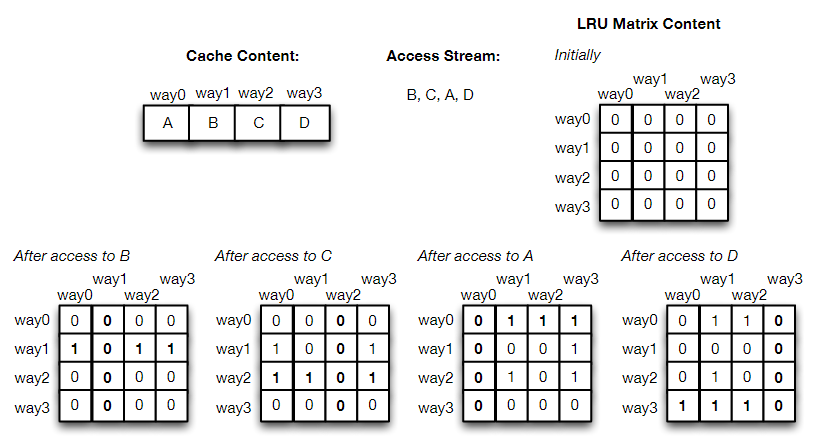
\includegraphics[width=\textwidth]{assets/lru-matrix-implementation.png}
	\end{figure}

	\subsubsection{Pseudo-LRU implementation}

	\begin{itemize}
		\item LRU implementation takes $O(way^2)$ space and time; too expensive
		\item PLRU approximates LRU with decent accuracy
		\item PLRU complexity is $O(way)$
	\end{itemize}

	\begin{figure}[ht!]
		\centering
		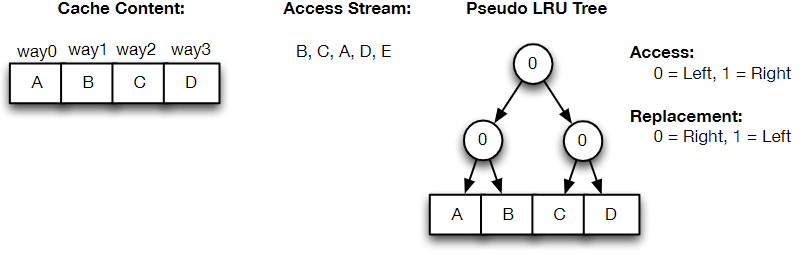
\includegraphics[width=\textwidth]{assets/plru-initial-state.png}
	\end{figure}

	\begin{figure}[ht!]
		\centering
		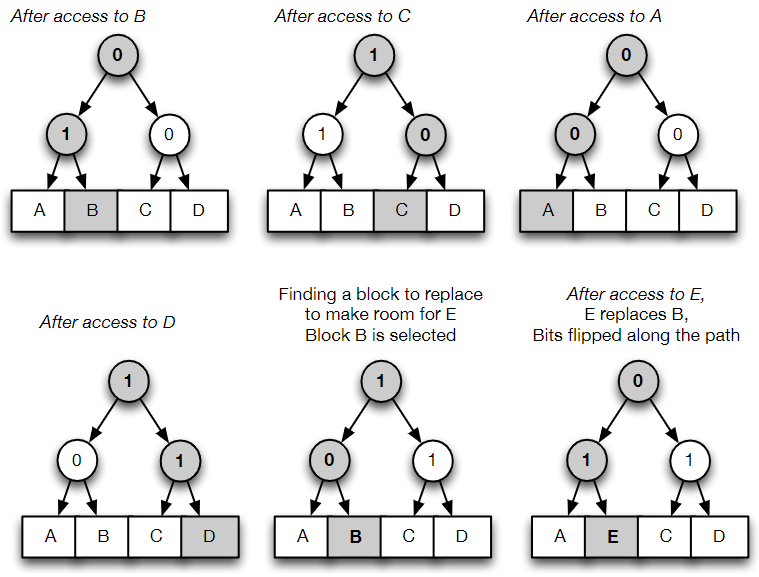
\includegraphics[scale=0.7]{assets/plru-walkthrough.png}
	\end{figure}

	\newpage

	\subsection{Inclusion Policies}

	\begin{itemize}
		\item block in inner cache level \textit{always} included in outer level cache too: \textbf{inclusive}
		\item block in inner cache level \textit{never} included in outer level cache too: \textbf{exclusive}
		\item block in inner cache level \textit{sometimes} included in outer level cache: \textbf{non-inclusive}
	\end{itemize}

	\begin{center}
		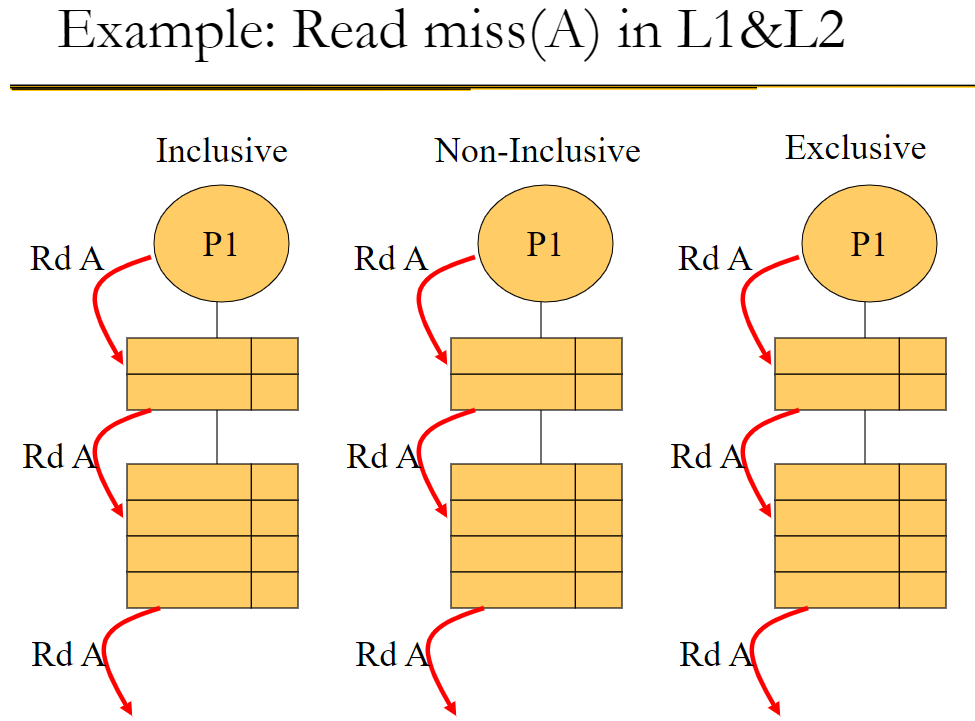
\includegraphics[scale=0.5]{assets/inclusion-policy-ex1.png}
		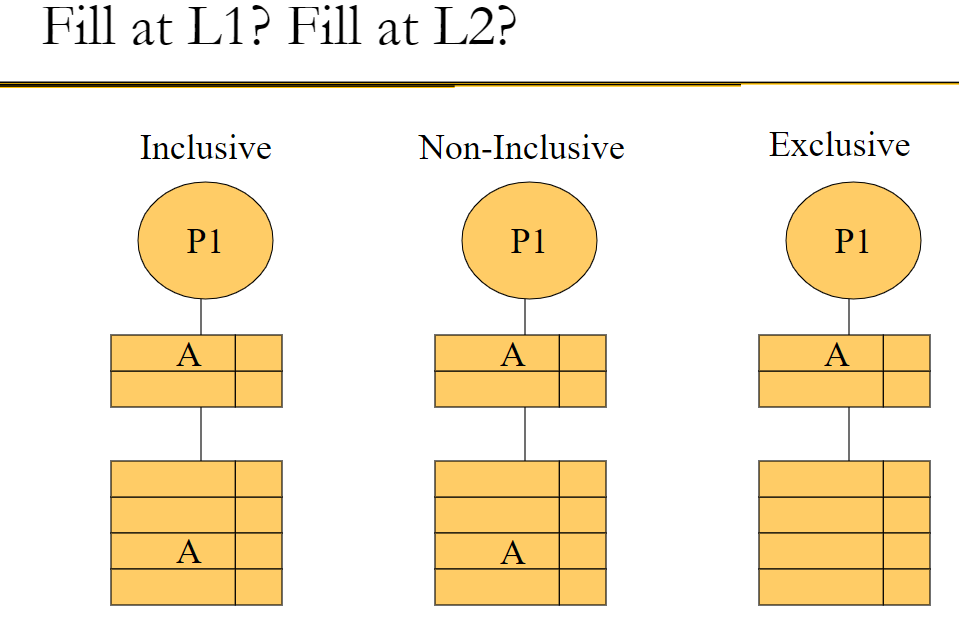
\includegraphics[scale=0.5]{assets/inclusion-policy-ex2.png}
		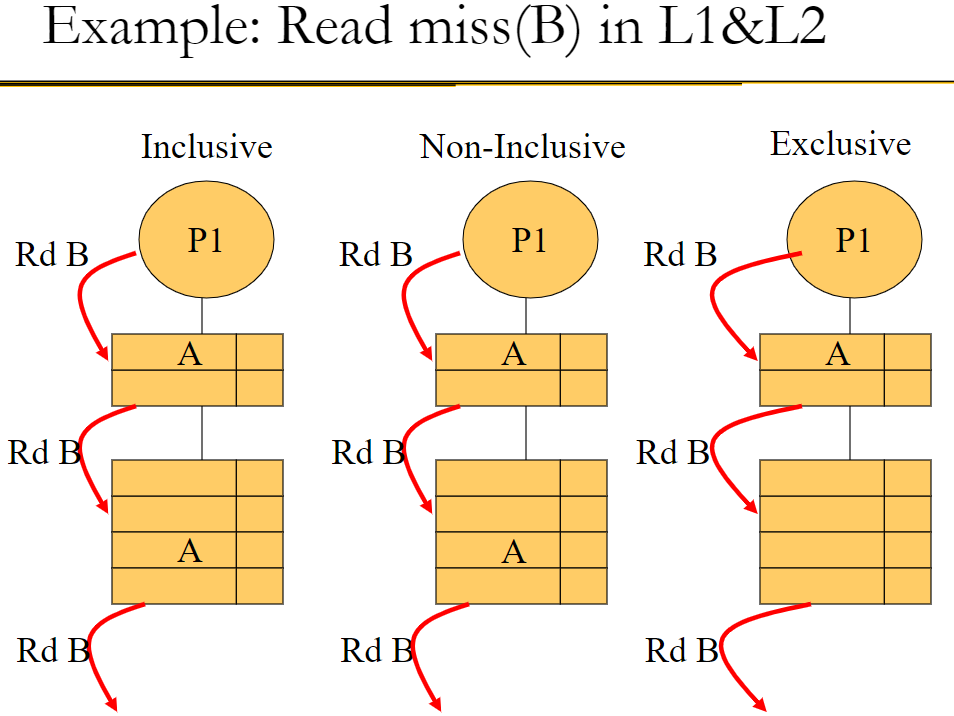
\includegraphics[scale=0.5]{assets/inclusion-policy-ex3.png}
		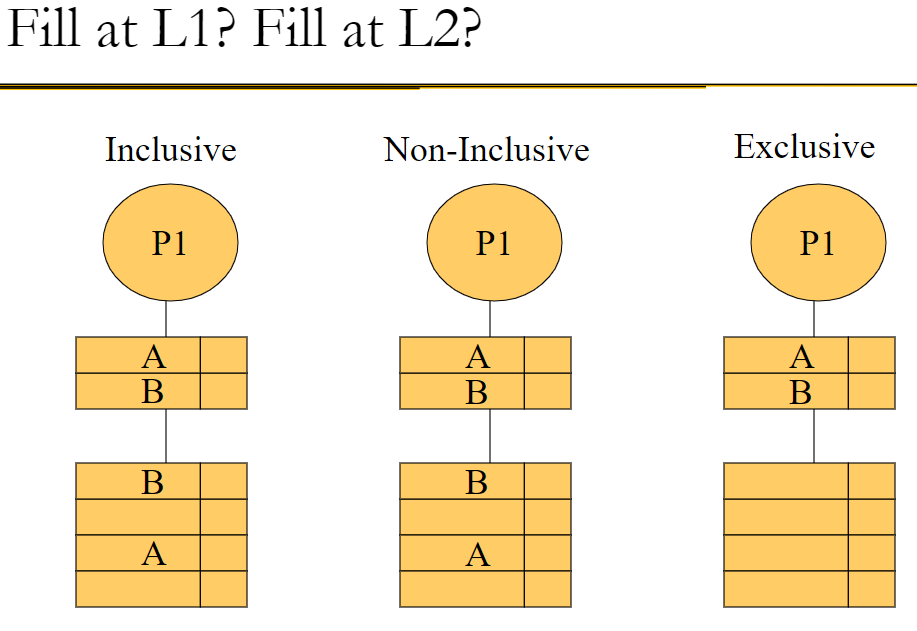
\includegraphics[scale=0.5]{assets/inclusion-policy-ex4.png}
		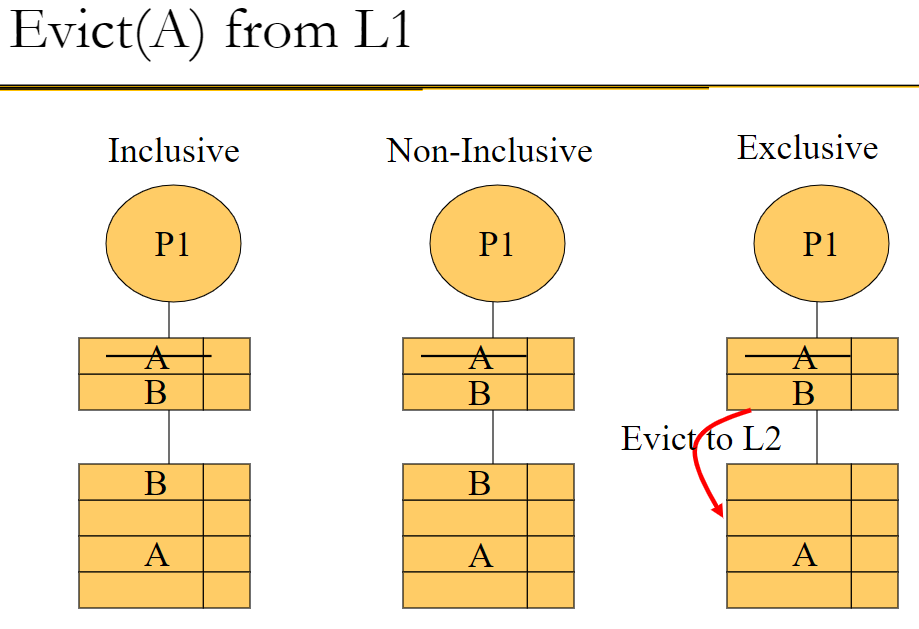
\includegraphics[scale=0.5]{assets/inclusion-policy-ex5.png}
		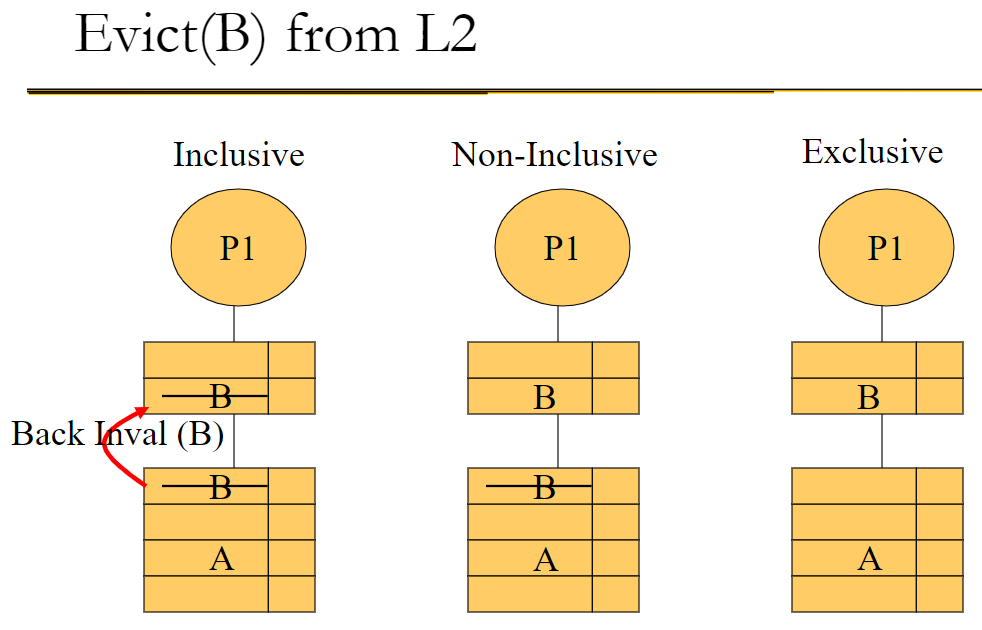
\includegraphics[scale=0.5]{assets/inclusion-policy-ex6.png}
	\end{center}

	\subsubsection{Inclusive outer cache Pros/Cons}

	Pros:

	\begin{itemize}
		\item for most cases, external requests can be checked against the outer cache (if not in outer, cannot be in inner)
		\item reduces contention for cache tags at inner cache
		\item external snoop latency (and thus memory latency) is reduced significantly
	\end{itemize}
	
	\noindent Cons:

	\begin{itemize}
		\item space wasteful; forced data redundancy
		\item inflexible (power gating ways makes inner cache ineffective)
	\end{itemize}

	\subsection{Cache Performance}

	\subsubsection{Performance Metrics}

	\begin{itemize}
		\item Average Access Time (AAT)
		\begin{itemize}
			\item $AAT = L_1T + L_1MR \cdot L_2T + L_1MR \cdot L_2MR \cdot L_2MT$
			\item $L_nT =$ level $n$ access time
			\item $L_nMR =$ level $n$ miss rate
			\item $L_nMT =$ level $n$ miss penalty
		\end{itemize}
	\end{itemize}

	\newpage

	\noindent CPI and AAT

	\begin{itemize}
		\item CPI (cycles per instruction) measures impact of AAT on overall performance
		\item CPU time = $CPI \cdot IC \cdot AAT$
		\item $CPI = CPI_0 + MemF \cdot AAT$
		\begin{itemize}
			\item $CPI_0$ = CPI with a perfect cache (0\% miss rate and 0-cycle access time)
			\item $MemF$ = fraction of instructions which are loads/stores
			\item the latencies used (i.e. $L_nMT$) must be ones that are \textit{not} overlapped with computation and 
			must be amortized over concurrent memory accesses (i.e. divide by number of simultaneous memory accesses)
		\end{itemize}
	\end{itemize}

	\subsubsection{Examples}

	Suppose that we have a system with two levels of caches. The L1 cache has an access latency of 1 clock cycle, while 
	the L2 cache has an access latency of 9 clock cycles. An L2 cache miss costs 100 clock cycles to service.
	
	\begin{enumerate}
		\item Calculate the average access time (AAT or AMAT) if an application suffers 20\% L1 miss rate and 10\% L2 miss rate.
		\item Calculate AAT' if it is known that on average, 100\% of L1 cache access latency is overlapped with computation, 
		50\% of L2 cache access latency is overlapped with computation, and 0\% L2 miss latency is overlapped with computation. 
		Assume that on average, 2 memory references are serviced simultaneously for L2 cache accesses, and only 1.2 for 
		L2 cache misses.
		\item Calculate the CPI using AAT' if the perfect cache CPI is 0.5 and 20\% of all instructions are memory 
		references (load/store).
	\end{enumerate}

	\noindent Answer:

	\begin{enumerate}
		\item use $AAT = L1T + L1MR \cdot L2T + L1MR \cdot L2MR \cdot L2MT$
		\begin{itemize}
			\item $AAT = 1 + 0.2 \cdot 9 + 0.2 \cdot 0.1 \cdot 100 = 1 + 1.8 + 2 = 4.8$ clock cycles
		\end{itemize}

		\item New AAT'
		\begin{itemize}
			\item $L_1T = 0$ (because it is completely overlapped with computation)
			\item $L_2T = \frac{0.5 \cdot 9}{2} = 2.25$
			\item $L_2MT = \frac{1.0 \cdot 100}{1.2} = 83.3$
			\item $AAT' = 0 + 0.2 \cdot 2.25 + 0.2 \cdot 0.1 \cdot 83.3 = 0.45 + 1.67 = 2.12$
		\end{itemize}

		\item use $CPI = CPI_0 + MemF  \cdot AAT'$
		\begin{itemize}
			\item $CPI = 0.5 + 0.2 * 2.12 = 0.92$
		\end{itemize}
	\end{enumerate}

	\subsection{Improving Cache Performance}

	\subsubsection{Reduce miss rate}

	Types of cache misses:

	\begin{itemize}
		\item compulsory: misses required to bring blocks into the cache for the first time
		\item conflict: misses that occur due to insufficient cache associativity
		\item capacity: misses that occur due to finite cache size
		\item coherence: misses that occur due to invalidation by other processors
		\item system related: misses due to system activities such as system calls, interrupts, context switches, etc.
	\end{itemize}

	\begin{tabular}[ht!]{|c|c|c|c|} \hline
		Parameters				& Compulsory	& Conflict		& Capacity		\\ \hline
		larger cache size		& unchanged		& unchanged		& reduced		\\ \hline
		larger block size		& reduced		& unclear		& unclear		\\ \hline
		larger associativity	& unchanged		& reduced		& unchanged		\\ \hline
	\end{tabular}

	\noindent Reducing miss rate:

	\begin{enumerate}
		\item increase block size
		\begin{itemize}
			\item (+) idea: exploit spatial locality
			\item (-) overdoing it can lead to cache pollution from useless data
			\item (-) also increases miss penalty (have to bring more data in each miss)
		\end{itemize}

		\item increase cache size
		\begin{itemize}
			\item (+) larger caches hold more
			\item (-) steals resources from other units
			\item (-) diminishing returns: double size != double performance
			\item (-) larger caches are slower to access
		\end{itemize}

		\item increase set associativity
		\begin{itemize}
			\item (+) fully associative yields better performance than direct mapped
			\item (-) slower (spend more time searching within a set)
			\item (-) diminishing returns: 8-way set-associative often comparable (almost equivalent) in HR/MR to fully-associative
		\end{itemize}

		\item hashing for better set mapping within cache
		\begin{itemize}
			\item useful if sets are not uniformly utilized (i.e. most of the time, addresses map to set index 0)
		\end{itemize}

		\item replacement or LRU insertion
		\begin{itemize}
			\item LRU works well 80\% of the time, but poorly when the working set is larger than cache
			\item replacement: detect pathological cases and use random replacement
			\item placement: detect pathological cases and insert at LRU
		\end{itemize}

		\item \textbf{Prefetching}
		\begin{itemize}
			\item prefetch: get data in cache before it's needed/requested by the processor
			\item important metrics:
			\begin{itemize}
				\item coverage: fraction of misses prefetched
				\item accuracy: fraction of prefetches that are useful
				\item timeliness: implicitly part of accuracy, but also important to consider
			\end{itemize}

			\begin{center}
				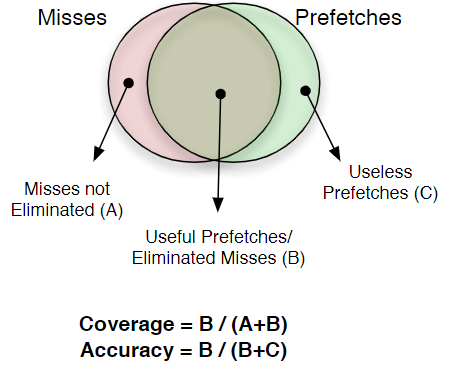
\includegraphics[scale=0.75]{assets/prefetching-metrics-diagram.png}
			\end{center}

			\item next line prefetching:
			\begin{itemize}
				\item fetch missing/requested block \textit{and} the next sequential block
				\item works great for stream with high sequential locality i.e. instruction caches (Icaches)
				\item uses unused memory bandwidth between misses (can hurt if there isn't much leftover bandwidth)
			\end{itemize}

			\item stride prefetching
			\begin{itemize}
				\item if memory is being accessed every $n$ locations, then just prefetch block + $n$
				\item for example, useful in a for loop that increments by $n$ each iteration
			\end{itemize}

		\end{itemize}

		\item other optimizations
		\begin{itemize}
			\item loop interchange: increase temporal locality by exchanging inner and outer loops (i.e. 2d for loop 
			should have $i$ outer, $j$ inner if accessing $arr[i][j]$)
			\item loop fusion: two loops with identical sets of iterations can be combined into one loop (duplicated things 
			in the first loop might be out of the cache by the time the second loop executes, so putting both in one loop 
			reduces the chances of this)
		\end{itemize}
	\end{enumerate}

	\subsection{Cache Performance Improvements cont.}

	\subsubsection{Reduce hit time}

	\begin{itemize}
		\item use small and simple caches: lower access time needed, and decreased power consumption)
		\item way prediction
		\begin{itemize}
			\item goal is to keep hit time as low as possible (i.e. approach direct-mapped cache hit time)
			\item use ``Predicted Next Way'' (PNW) bits for each block
			\item when a block is accessed, read along its PNW bits
			\item on the next access, only read the predicted way (which is just a single tag comparison)
			\item if predicted correctly, you benefit from an extremely fast hit time; 90\% acc. for 2-way, 80\% for 4-way
			\item if predicted incorrectly, you pay the penalty of accessing other ways and then also having to update 
			the PNW bits
		\end{itemize}

		\item pipelined cache access: just pipeline the stages for accessing in a cache (decode \& activate row, tag compare, select bytes/words)
		\item split and multi-banked cache organization
		\begin{itemize}
			\item in a unified L1 cache that holds instructions and data, each cycle it has to be accessed to supply instructions 
			to the pipeline, and each cycle, several load/store instructions may access it. Thus, it needs to have many ports 
			(expensive and slow)
			\item solution: split into instruction cache + data cache
			\item no longer contending for the same ports
			
			\begin{center}
				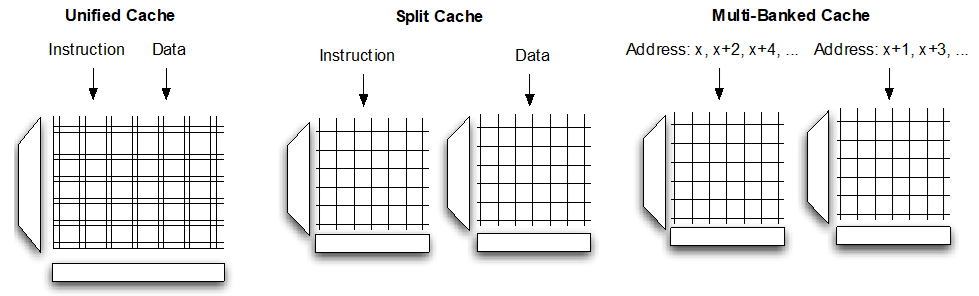
\includegraphics[scale=0.6]{assets/unified-split-multibank.png}
			\end{center}
		\end{itemize}

	\end{itemize}

	\subsubsection{Reduce miss penalty}

	\begin{itemize}
		\item use multi-level caches
		\begin{itemize}
			\item single level cache: too small, high miss rate; too large, high hit (access) time
			\item multi-level cache: L1 (small but fast), L2 (slower but larger), L3 (even slower but even larger)
			\item since it takes a long time to go down to main memory, just put a cache between L1 and main memory (L2 cache)
		\end{itemize}

		\item use write buffers
		\begin{itemize}
			\item for writes (write-through) or write backs (write-back), don't make CPU wait on the write to memory
			\item use a write buffer: on read miss, check for match
		\end{itemize}

		\item early restart/critical word first
		\begin{itemize}
			\item early restart: as soon as requested word arrives, forward it to CPU; miss penalty time is now the time 
			needed to fetch the requested word
			\item critical word first: problem with early restart (what if requested word is in the middle of a block?); 
			start fetching the block with the required (critical) word, and fill in the rest
		\end{itemize}

		\item subblocking
		\begin{itemize}
			\item problem: tags are overhead, and take up extra space
			\item partial soln: large blocks reduce amount of tag storage (double blocksize means we halve the num. blocks, 
			which also means we halve the number of tags); but large blocks increase miss penalty
			\item complete soln: use large blocks, but also subdivide blocks into subblocks. Fetch only 1 subblock on a miss, 
			keep valid bit for subblocks. Also better if other subblocks are prefetched in the background (aka combine 
			subblocking with early restart/critical word first)
		\end{itemize}
	\end{itemize}

	\subsubsection{Reduce power consumption}

	\begin{itemize}
		\item parallel vs. sequential cache access: parallel is faster, but sequential is more power efficient; use parallel 
		for L1, and sequential for L2/L3
	\end{itemize}

	\subsection{Virtual Memory}

	Program uses virtual address but translates (maps) it to a physical address at runtime.

	\subsubsection{Paging}

	\begin{itemize}
		\item memory divided into chunks called pages, typically 4KB
		\item each page in program address space mapped into a page frame
		\item page has virtual address (VA), page frame has physical address (PA)
		\item OS keeps a page table that translates VA to PA; each entry is a page table entry (PTE)
		\item illusion of larger memory than physically available by swapping space in storage (page swapped in/out on demand)
	\end{itemize}

	\subsubsection{Page fault}

	\begin{itemize}
		\item page fault: exception raised because of illegal access (insufficient permission [write to read-only], page miss 
		[page not in physical memory due to PTE being unmapped])
		
		\item page miss handling:
		\begin{itemize}
			\item page miss incurs a page fault, triggers OS page fault handler
			\item victim page selected and swapped out to swap space in disk
			\item page read from disk and swapped into now-free page frame
			\item page fault handler exits, and instruction that caused page fault re-executed
		\end{itemize}
	\end{itemize}

	\subsubsection{Accelerating page table access}

	\begin{itemize}
		\item page table is large, so accessing it takes a while
		\item use a cache of a small number of PTEs that are recently used, called a Translation Lookaside Buffer (TLB)
		\item just like regular caches, a TLB can have/be:
		\begin{itemize}
			\item split into instruction and data TLB
			\item multi-level
			\item replacement policies (LRU, PLRU, etc.)
			\item associativity, blocksize, cache size is fixed to size of PTE
		\end{itemize}
	\end{itemize}

	\subsubsection{Page table size}

	\begin{itemize}
		\item suppose we have a 48-bit address space, and page size is 4KB (hence 12-bit page offset)
		\item there are $48 - 12 = 36$ bits used for page address
		\item so there are $2^{36} = 64$ giga pages
		\item each PTE is 8 Bytes in size, so page table is 64G $\cdot$ 8B = 512GB
		\item each program has a page table, so we need $1000 \cdot 512$GB for page tables normally; reduce this using 
		hierarchical page tables
	\end{itemize}

	\section{ILP Techniques: Pipelining}

	\subsection{Pipeline Design}

	\subsubsection{How to execute an instruction}

	5 stages:

	\begin{enumerate}
		\item Instruction fetch (IF)
		\begin{itemize}
			\item instruction register (IR) = Mem[PC]
			\item new PC = PC + 4
		\end{itemize}

		\item instruction decode/register fetch (ID)
		\begin{itemize}
			\item A = Regs[IR$_{6..10}$]
			\item B = Regs[IR$_{11..15}$]
			\item Imm = sign-extend(IR$_{16..31}$)
		\end{itemize}

		\item execute (EX)
		\begin{itemize}
			\item memory reference: ALU output = A + Imm
			\item reg/reg ALU operation: ALU output = A $op$ B
			\item reg/immediate ALU operation: ALU output = A $op$ Imm
			\item branch: ALU output = new PC + Imm; Cond = (A $op$ 0)
		\end{itemize}

		\item memory access/branch completion (MEM)
		\begin{itemize}
			\item memory reference
			\begin{itemize}
				\item \texttt{load\_mem\_data = Mem[ALUOutput] // load}
				\item \texttt{Mem[ALUOutput] = B  // store}
			\end{itemize}

			\item branch
			\begin{itemize}
				\item \texttt{if (cond) PC = ALUOutput; else PC = NPC}
			\end{itemize}
		\end{itemize}

		\item write-back (WB)
		\begin{itemize}
			\item reg-reg ALU operation: Regs[IR$_{16..20}$] = ALUOutput
			\item reg-immediate ALU operation: Regs[IR$_{11..15}$] = ALUOutput
			\item load instruction: Regs[IR$_{11..15}$] = \texttt{load\_mem\_data}
		\end{itemize}
	\end{enumerate}

	\noindent Pipeline speedups (no stalls) for a pipeline of $n$ stages

	speedup = $\frac{\texttt{avg. exec time unpipelined}}{\texttt{avg. exec time pipelined}}$

	speedup = $\frac{T_{unpipe}}{T_{unpipe} / n + T_{latch} \cdot (n - 1)} = n$ (ideal case, $T_{latch} = 0$)

	\begin{itemize}
		\item pipelining helps by keeping CT constant, while improving CPI
		\item or by keeping CPI constant, while improving CT
		\item but most of the time, pipelining does a bit of both improving CPI and CT
	\end{itemize}

	\subsubsection{Pipeline hazards}

	Three kinds:

	\begin{itemize}
		\item data hazards: dependencies between instructions prevent their overlapped execution
		\item structural hazards: not enough hardware resources for all combinations of instructions (i.e. two multiply 
		instructions need to be pipelined, but we only have one multiplier unit)
		\item control hazards: branches change the PC, which results in late code (if the wrong code is executed)
	\end{itemize}

	\subsection{Branch Prediction 1}

	Idea: avoid branch stalls by predicting which way a branch will go (i.e. taken vs. not-taken)

	\begin{itemize}
		\item perhaps use a prediction bit if branch taken, 0 if not taken. At instruction fetch, if prediction field is 1, 
		predict taken, else not taken.
		\item problem: some branches may alternate or not do the same thing every time, so we need more sophistication
	\end{itemize}

	\subsubsection{Smith $n$-bit counter predictor}

	Idea: replace prediction bit/field with an $n$-bit counter

	\begin{center}
		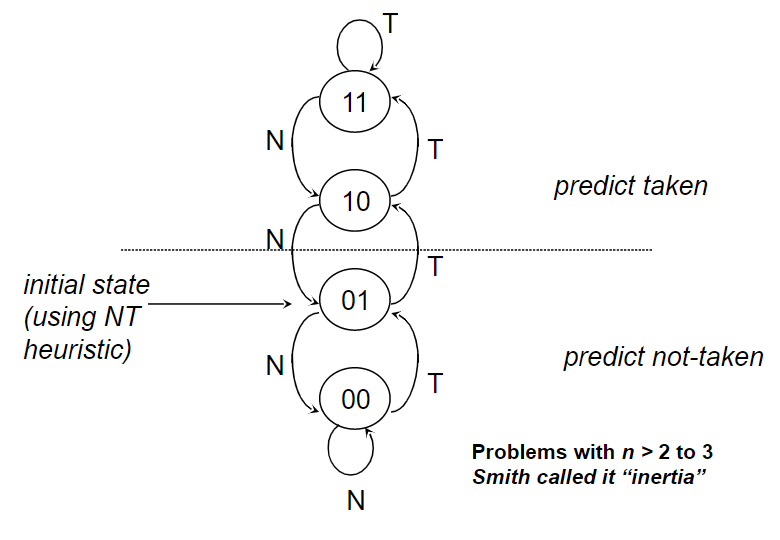
\includegraphics[scale=0.5]{assets/smith-counter.png}
	\end{center}

	\noindent Smith counter example (note the weakness on the alternating example):

	\begin{center}
		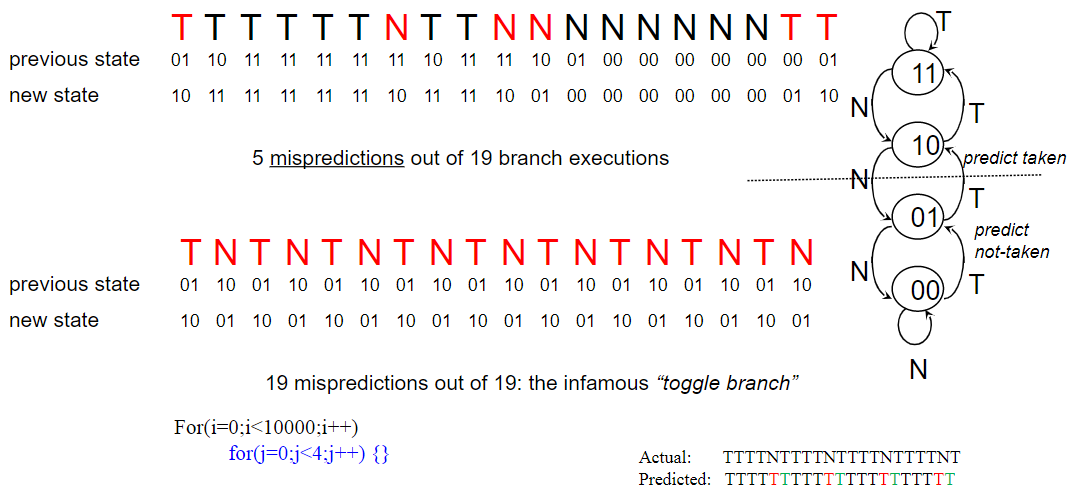
\includegraphics[scale=0.6]{assets/smith-example.png}
	\end{center}

	\subsubsection{Global Branch Correlation and Two-Level Global Branch Prediction}

	Associate branch outcomes with a global taken/not-taken history of all branches. Make a prediction based on the outcome 
	of the branch the last time the same global branch history was encountered.

	\begin{center}
		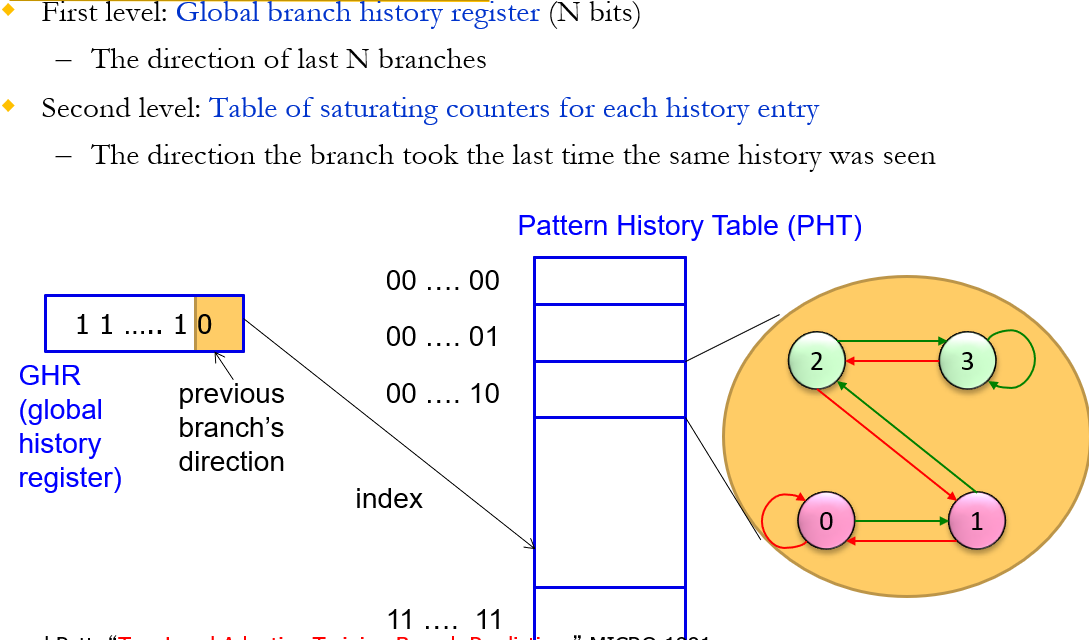
\includegraphics[scale=0.5]{assets/two-level-global-branch-pred.png}
	\end{center}

	\subsubsection{Gshare predictor}

	Problem with two-level global branch predictor was that prediction was only based on the global history of all branches, 
	independent of individual branches. Gshare adds more context by also considering individual branches (using both PC and 
	global branch history register to index into the pattern history table).

	\begin{center}
		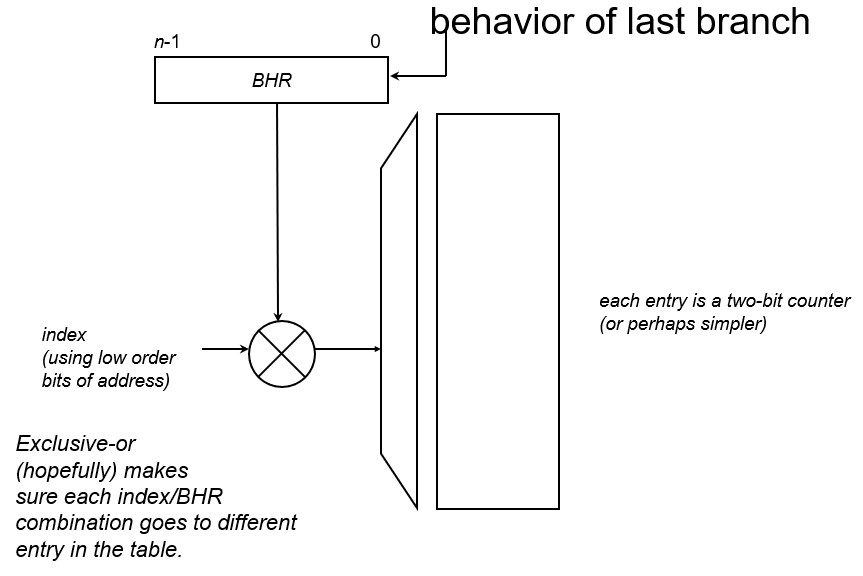
\includegraphics[scale=0.5]{assets/gshare-diagram.png}
	\end{center}

	\begin{center}
		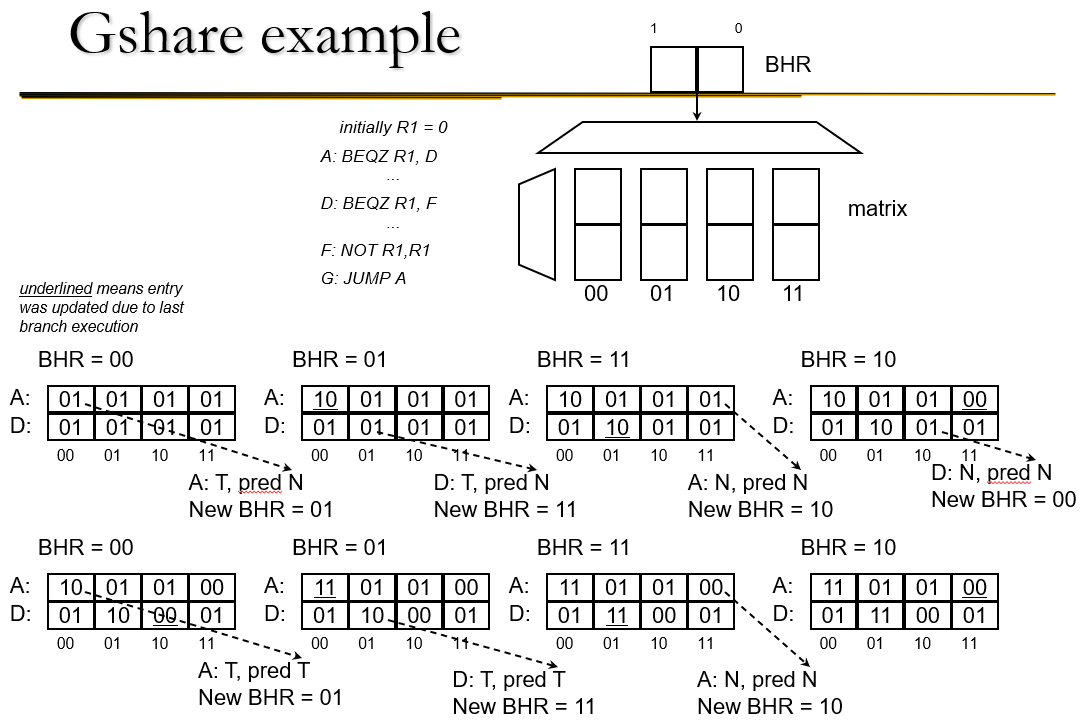
\includegraphics[scale=0.52]{assets/gshare-example.png}
	\end{center}

	\subsection{Branch Prediction 2}

	\subsubsection{Two-Level Local Branch History}

	Improving on Gshare: Local history with the Yeh/Patt Two-Level Local Branch predictor

	\begin{center}
		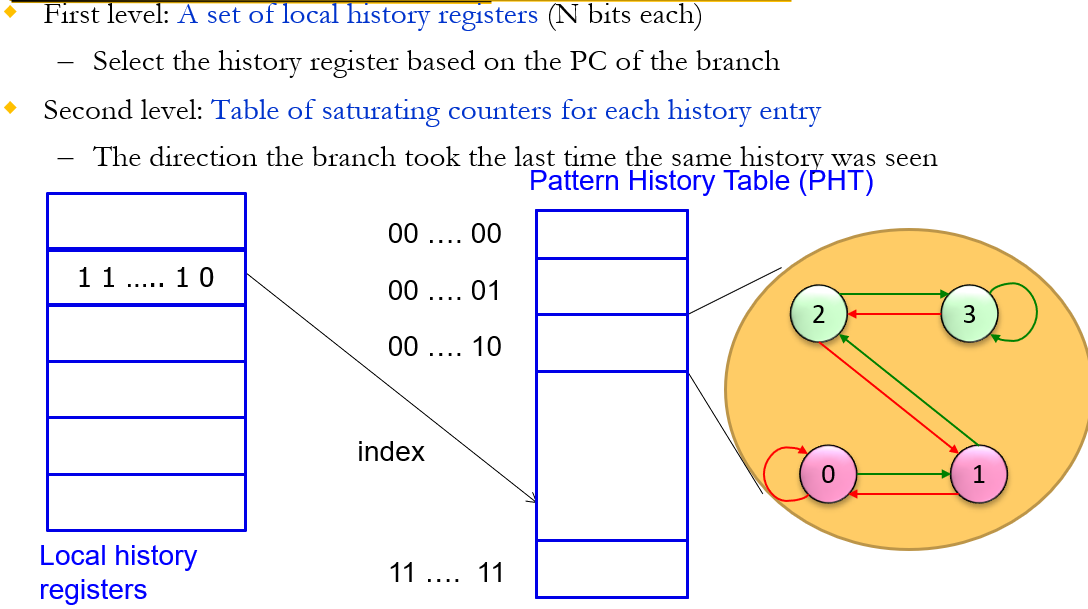
\includegraphics[scale=0.5]{assets/yeh-patt-diagram.png}
		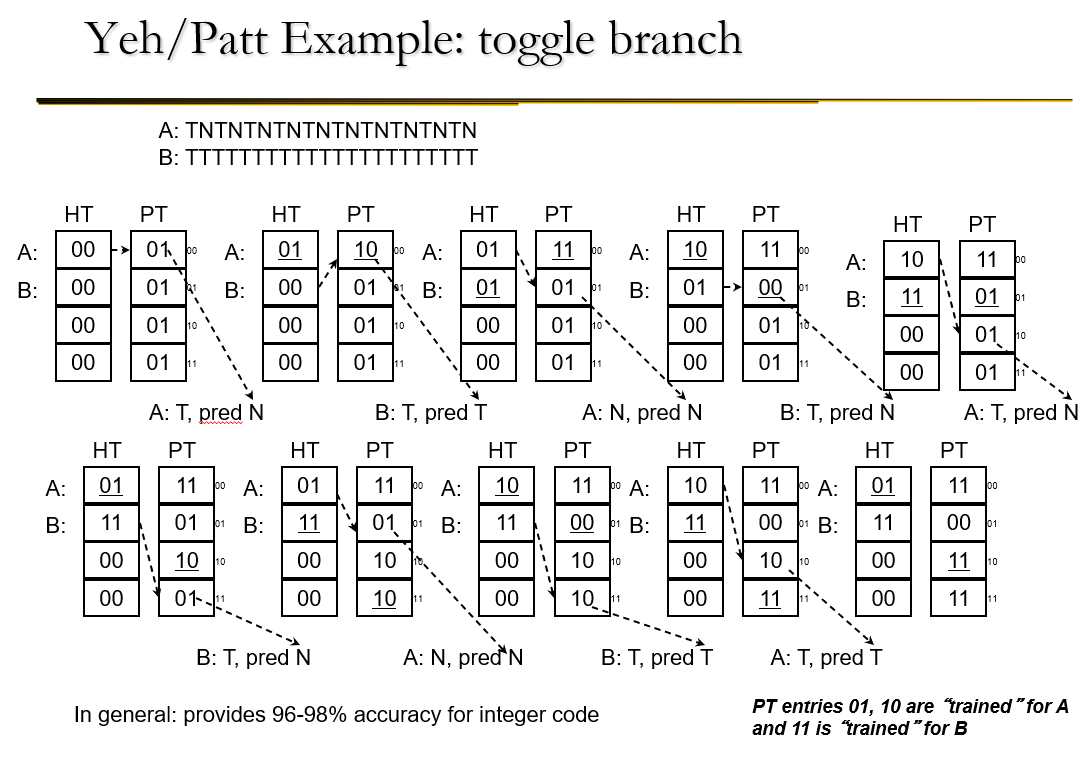
\includegraphics[scale=0.5]{assets/yeh-patt-example.png}
	\end{center}

	\subsubsection{Hybrid/Tournament predictors}

	There is no one-size-fits-all solution to branch prediction; some are just better for some programs while worse in 
	others. So, the idea is to use a combination of them, pick the one that is correct more often, and over time lean/have 
	a bias toward that one.

	\begin{center}
		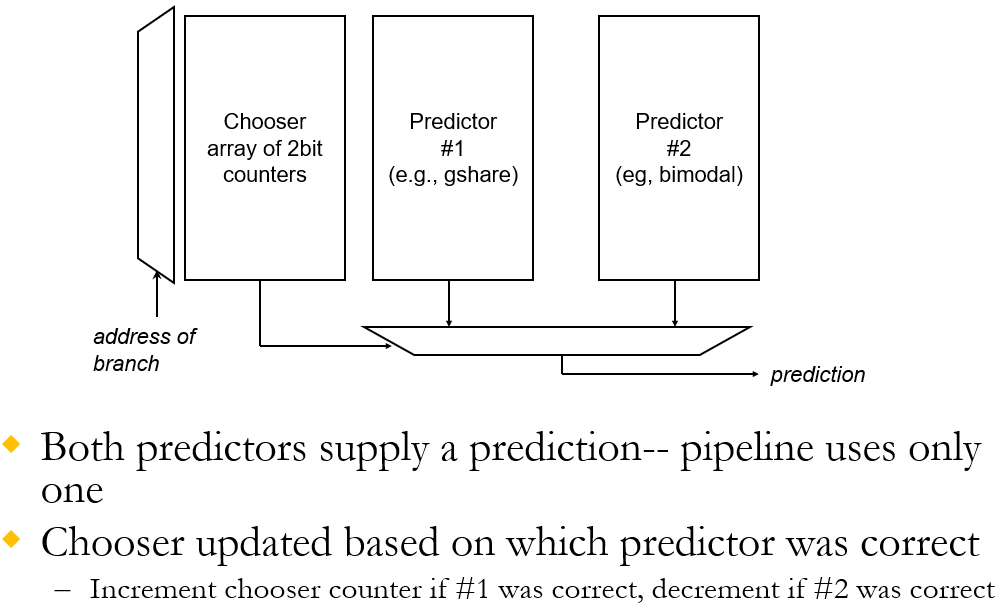
\includegraphics[scale=0.5]{assets/hybrid-example.png}
	\end{center}

	\subsection{Dependence Hazards and Pipeline Performance}

	\subsubsection{Types of dependencies}

	\begin{itemize}
		\item True dependence
		\begin{itemize}
			\item \texttt{ADD \underline{R1}, R2, R3}
			\item \texttt{SUB R4, R5, \underline{R1}}
			\item may cause \textbf{RAW} hazards
		\end{itemize}

		\item Anti-dependence
		\begin{itemize}
			\item \texttt{ADD R3, R2, \underline{R1}}
			\item \texttt{SUB \underline{R1}, R4, R5}
			\item may cause \textbf{WAR} hazards
			\item due to reuse, can be removed by just using another register
		\end{itemize}

		\item Output-dependence
		\begin{itemize}
			\item \texttt{ADD \underline{R1}, R2, R3}
			\item \texttt{SUB \underline{R1}, R4, R5}
			\item may cause \textbf{WAW} hazards
			\item due to reuse, can be removed by just using another register
		\end{itemize}
	\end{itemize}

	\subsubsection{Pipeline performance and loop analysis}

	\begin{center}
		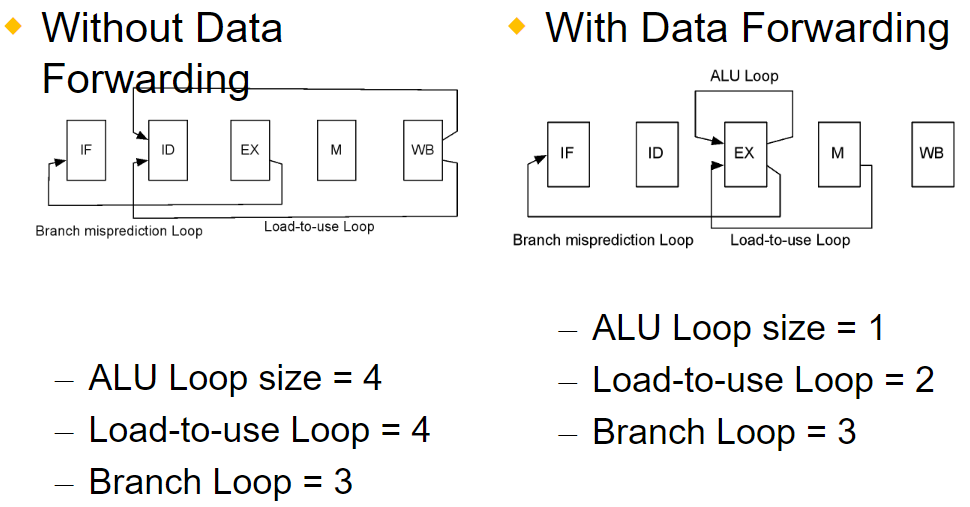
\includegraphics[scale=0.5]{assets/loop-analysis-ex1.png}
	\end{center}

	\begin{center}
		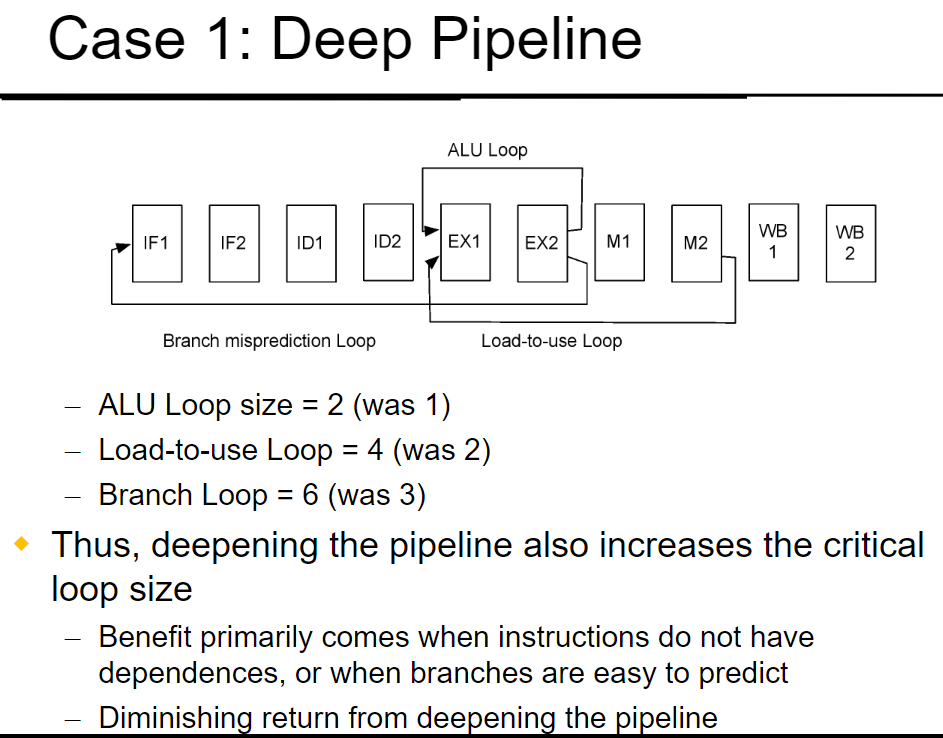
\includegraphics[scale=0.5]{assets/loop-analysis-ex2.png}
	\end{center}

	\begin{center}
		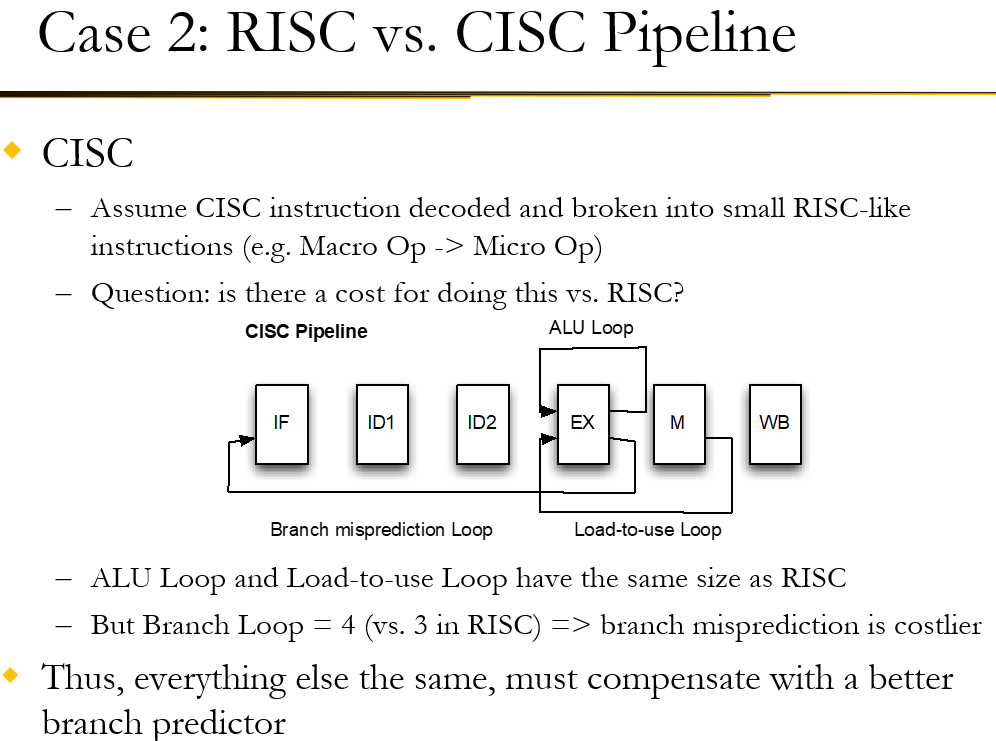
\includegraphics[scale=0.5]{assets/loop-analysis-ex3.png}
	\end{center}

	\begin{center}
		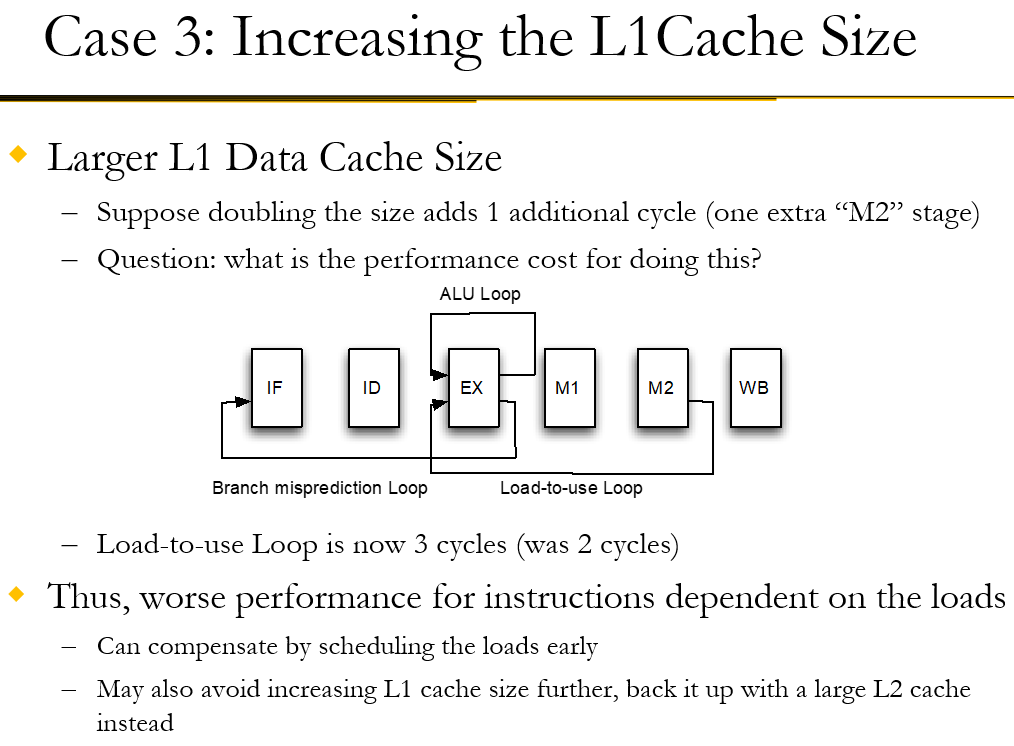
\includegraphics[scale=0.5]{assets/loop-analysis-ex4.png}
	\end{center}

\end{document}
